\chapter{Revisão Teórica}

\section{Vídeo Digital}
Como consta em \cite{h264avcs}, vídeo digital é a representação de uma cena do mundo real, amostrada espacialmente e temporalmente. Tipicamente uma cena é amostrada em um certo ponto no tempo para produzir um quadro, que representa a cena inteira naquele ponto no tempo. A amostragem é realizada em intervalos (ex. 1/25 ou 1/30 vezes por segundo).

Uma cena do mundo real costuma ser composta de múltiplos objetos, cada um com suas próprias características como forma, profundidade, textura e iluminação. A cor e o brilho de uma cena pode variar com diferentes graus de lisura ao longo da cena. As características de uma cena mais relevantes para o processamento e compressão de vídeo incluem características espaciais como variação de textura na cena, quantidade de forma dos objetos, cor, etc, e características temporais como o movimento de um determinado objeto, mudanças na iluminação e no movimento da câmera.

Usualmente uma cena é amostrada espacialmente sendo representada como uma grade retangular ou quadrada, o número de pontos amostrados no momento da captura influência a qualidade final da imagem. Essa quantidade de pontos amostrados normalmente é chamada de resolução da imagem. 

Uma vídeo em movimento é formado por se tirar "retratos" retangulares do sinal analógico que está sendo capturado em intervalos de tempo periódicos. Reproduzir uma série desses retratos ou quadros produz uma aparência de movimento. Uma taxa de amostragem alta fornece uma aparência de movimento mais suave, mas requer que mais amostras sejam capturadas e armazenadas.


\subsection{Espaços de cor}

A maior parte das aplicações de vídeo precisam representar cores, portanto precisam de um mecanismo de captura e representação de informações de cor. Uma imagem monocromática requer apenas um número para indicar o brilho ou luminância de cada amostra espacial. Porém imagens coloridas necessitam de no mínimo três números por pixel para representar a cor de forma precisa. O método escolhido para representar brilho, luminância ou luma e cor é descrito como espaço de cor.

Um dos espaços de cor mais conhecidos é o RGB, nesse formato uma amostra de imagem colorida é representada por três números que indicam a porção de vermelho, verde e azul, as 3 cores primárias. Combinar essas três cores pode produzir qualquer outra cor, dessa maneira o espaço de cor RGB consegue capturar e exibir imagens coloridas com sucesso. Capturar uma imagem RGB envolve filtrar os componentes vermelho, verde e azul de cada cena sem sensores separados (normalmente são utilizados CCDs na captura de imagens). Displays coloridos exibem uma imagem RGB por iluminarem o componente vermelho, verde e azul de cada pixel de acordo com a intensidade de cada componente de cor. De uma distancia normal, esses componentes separados se misturam e formam a aparência de uma cor de verdade.

Apesar de também ser muito utilizado, o espaço de cor RGB não é o mais bem adaptado a visão humana, que é mais sensível a luminância do que a cor, dessa maneira o RGB acaba ignorando informações importantes para a visão humana (luminância) e armazenando outras menos importantes (cores). É possível guardar uma cor de maneira mais eficiente por separar a informação de luminância da informação de cor e representar a informação de luminância (também chamada de luma) com um resolução mais alta.

O espaço de cor Y:Cr:Cb normalmente é utilizado para representar cores de forma eficiente, otimizando as informações para serem mais relevantes à visão humana. Nesse espaço de cor o Y representa a luminância e pode ser calculado como a média ponderada dos valores do canal R,G e B.

\begin{equation}
Y = krR + kgG + kbB
\end{equation} 

onde k são os pesos para cada canal.

A informação de cor pode ser representada como componentes de diferença de cor (crominância ou croma). Onde cada componente de crominância é a diferença entre R,G ou B e a luminância Y:

\begin{equation}
Cr = R - Y
\end{equation}

\begin{equation}
Cb = B - Y
\end{equation}

\begin{equation}
Cg = G - Y
\end{equation}


Como Cr + Cb + Cg é uma constante somente dois dos valores de crominância precisam ser armazenados ou transmitidos, já que o terceiro componente pode ser calculado a partir dos outros dois. No Y:Cr:Cb somente o luma (Y) e o croma vermelho e azul são transmitidos. Os componentes de croma Cr e Cb podem ser representados com uma resolução menor que o luma já que o olho humano é menos sensível à cor do que a luz. Dessa maneira reduzimos a quantidade necessária para representar os componentes de crominância sem ter efeitos muito óbvios na qualidade visual.

O Y:Cr:Cb possui três modos de amostragem suportados pelo H.264, esses modos são o 4:2:0, 4:2:2, 4:4:4. Os números indicam a taxa de amostragem de cada componente na direção horizontal. No 4:4:4 para cada quatro amostras de luminância tempos quatro Cr e quatro Cb, no 4:2:2, também conhecido como YUY2, os componentes de crominância possuem a mesma resolução vertical que a luminância mas metade da resolução horizontal, 4:2:2 significa assim que para cada quatro amostras de luminância na direção horizontal existem duas amostras de Cr e duas de Cb. 4:2:2 normalmente é utilizado para reprodução de vídeos em alta qualidade de cor.

O formato mais popular para codificação de vídeo, normalmente utilizado em aplicações como vídeo conferência, televisão digital e DVD é o 4:2:0, também conhecido como YV12, Cr e Cb possuem metade da resolução horizontal e vertical do Y. Cada componente de cor possui um quarto das amostras que existem no componente luma, dessa maneira um vídeo 4:2:0 necessita da metade das amostras necessárias em um vídeo 4:4:4 ou RGB.

\section{Codificação de Vídeo Digital}

Como consta em \cite{h264avcs}, compressão é o ato ou processo de compactar dados em um menor número de bits que o original. Compressão de vídeo é o processo de converter vídeo digital em um formato mais adequado para envio ou armazenamento. A compressão baseia-se na remoção de redundância, removendo assim componentes que não são necessários para a reprodução do vídeo, normalmente utiliza-se uma abordagem de compactação com perda, buscando remover redundância temporal e espacial.

No domínio temporal existe uma alta correlação entre quadros que foram capturados em instantes similares de tempo, principalmente quando a taxa de amostragem é alta, existindo muita informação redundante que pode ser removida entre esses quadros. No domínio espacial existe uma correlação entre os pixels que estão perto um do outro, sendo mais uma fonte de informações redundantes que pode vir a ser comprimida.

Por isso normalmente os modelos de CODEC, como o H.264, MPEG-2 Vídeo, MPEG-4 Visual, H.263, VC-1, etc, utilizam predição e/ou compensação de movimento para remover redundância inerente tanto no próprio quadro (espacial) como entre quadros (temporal). Este trabalho é realizado no módulo de predição que tem por objetivo formar uma predição do quadro e então subtrair a predição deste mesmo quadro, gerando assim uma amostra residual do quadro. A predição pode ser formada a partir de quadros que já foram processados (nesse caso ela é temporal) ou a partir de amostras já processadas do mesmo quadro (nesse caso ela é espacial).

Quanto menos energia existir na amostra residual gerada, melhor terá se saído o módulo de predição. Para realizar a predição o codificador deve utilizar apenas informações que estão disponíveis ao decodificador, ou seja, dados que já foram codificados e transmitidos, senão o decodificador não será capaz de reconstruir o quadro, pois ele necessita recriar a mesma predição feita no codificador para adicioná-la ao resíduo recebido e gerar o quadro.

Com exceção de regiões descobertas e mudanças drásticas de iluminação, a maior parte das diferenças que ocorrem entre os quadros de um vídeo se dá pelo movimento dos pixels entre os quadros, dessa maneira é possível calcular a trajetória de cada pixel entre sucessivos quadros do vídeo, gerando uma matriz de vetores de movimento para cada pixel. Porém realizar com precisão esse cálculo para cada pixel exige um esforço computacional muito grande, se tornando impraticável. Para contornar esse problema a estimativa e compensação de movimento é realizada em macro blocos e não por pixel.

\subsection{Predição de um macrobloco utilizando compensação de movimento}

O macrobloco, que normalmente corresponde a uma região de 16 x 16 pixels de um quadro, é a unidade básica do processo de predição por compensação de movimento em vários padrões de codificação de vídeo como MPEG-1, MPEG-2, MPEG-3, MPEG-4 Visual, H.261, H.263 e H.264. Um macrobloco no formato de vídeo mais comum, que é o 4:2:0, é formado por uma região de 16 x 16 pixels, onde temos 256 amostras de luminância organizadas em 4 blocos de 8 x 8 pixels, 64 amostras de crominância vermelha em um bloco de 8 x 8 pixels e 64 amostras de crominância azul também arranjadas como um bloco de 8 x 8. No H.264 cada quadro de vídeo é processado como um conjunto de macroblocos.


\subsection{Estimativa de movimento}

A estimativa de movimento de um macrobloco envolve,a partir de um quadro de referência previamente selecionado, encontrar uma região 16 x 16 neste quadro que seja o mais semelhante possível com o macrobloco atual. O quadro de referência deve ser um quadro que já foi codificado e deve ser anterior ou posterior ao quadro atual em relação a ordem de amostragem. A partir da posição do macrobloco corrente define-se uma área de busca por uma outra região que se assemelhe a ele no quadro de referência, dentro dessa área de busca procura-se a região de 16 x 16 que mais se assemelha com o macrobloco.


\subsection{Compensação de movimento}

As amostras de luminância e crominância da região selecionada no quadro de referência são subtraídas do macrobloco corrente para produzir um macrobloco residual que é codificado e transmitido junto com um vetor de movimento descrevendo a posição da região selecionada em relação a posição do macrobloco corrente.

Existem variações no processo de estimativa e compensação de movimento. O quadro de referência pode ser um quadro anterior, posterior ou uma combinação da predição de dois ou mais quadros que já foram codificados. Se um quadro posterior ao corrente é selecionado, é necessário codificar esse quadro antes que o corrente, ou seja os quadros terão de ser codificados fora da ordem de apresentação. Quando ocorre uma mudança brusca entre o quadro de referência e o quadro corrente, por exemplo uma grande área foi descoberta, pode ser mais eficiente codificar o macrobloco sem realizar a compensação de movimento. Dessa maneira o codificador pode utilizar predição interna (espacial) ou a predição externa com compensação de movimento para cada macrobloco de acordo com a situação do quadro corrente. 


\section{MPEG 4 Parte 10}

O MPEG 4 Parte 10 (também conhecido como H.264 ou AVC) é um padrão de compressão de vídeo. \cite{ituh264avc} é um documento publicado por duas organizações padronizadoras, a ITU-T e a ISO/IEC. Um codificador H.264 funciona realizando predição, transformação e codificação do resultado final, produzindo assim um bitstream. O decodificador realiza o processo complementar, decodificando a informação, realizando uma transformada inversa e reconstrução dos quadros previamente codificados.


\begin{figure}[H]
\centering
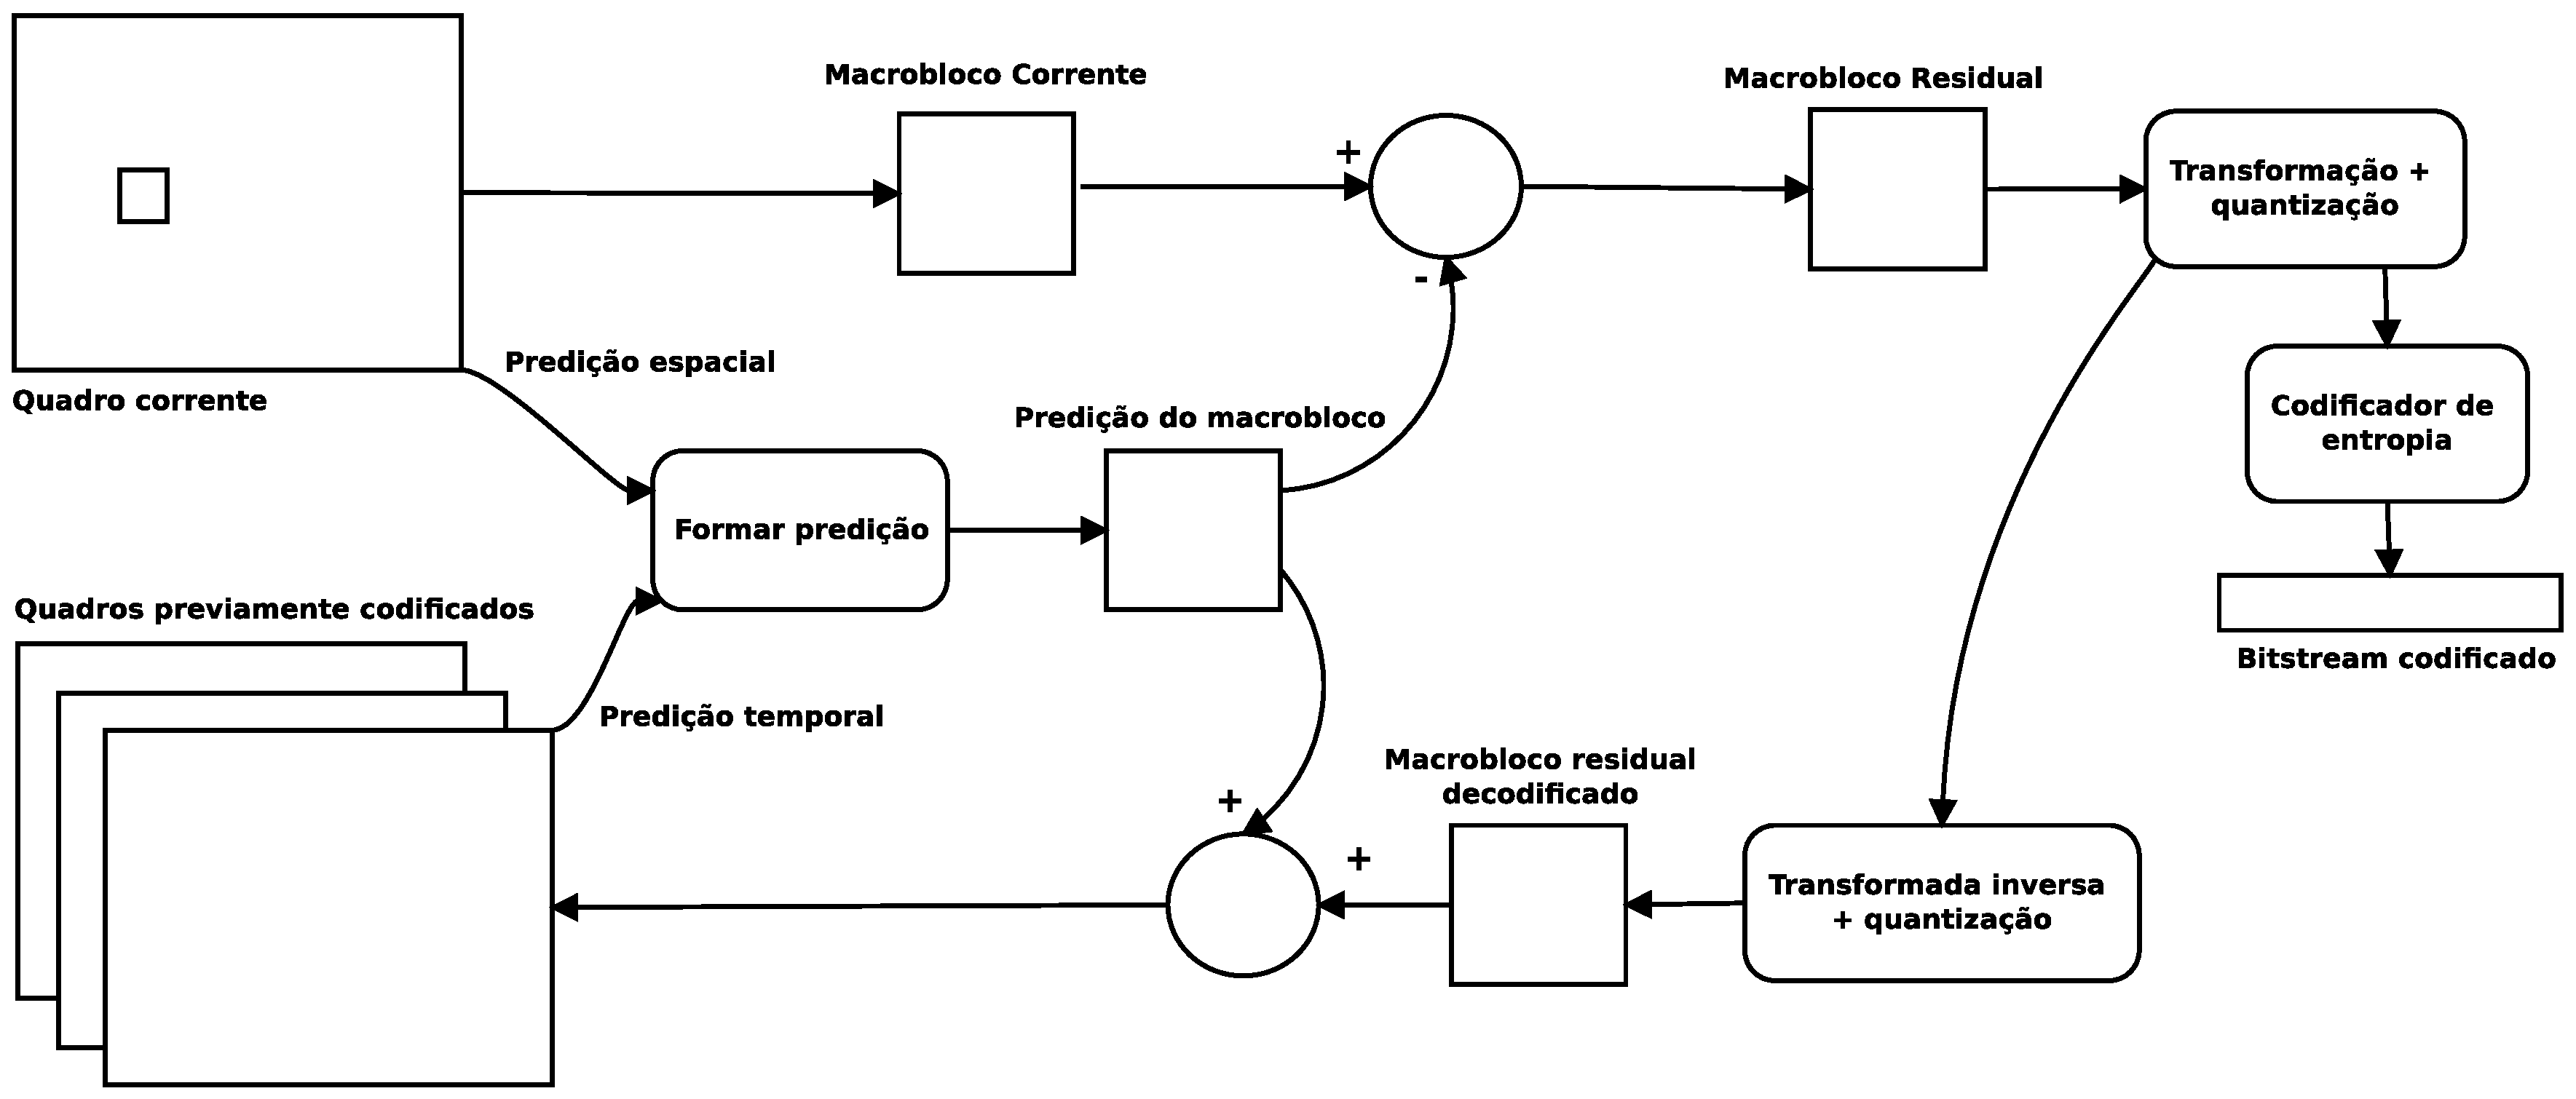
\includegraphics[scale=0.3]{imagens/fig1.eps}
\caption{Típico codificador H.264}
\label{fig:h264_encoder}
\end{figure}


\begin{figure}[H]
\centering
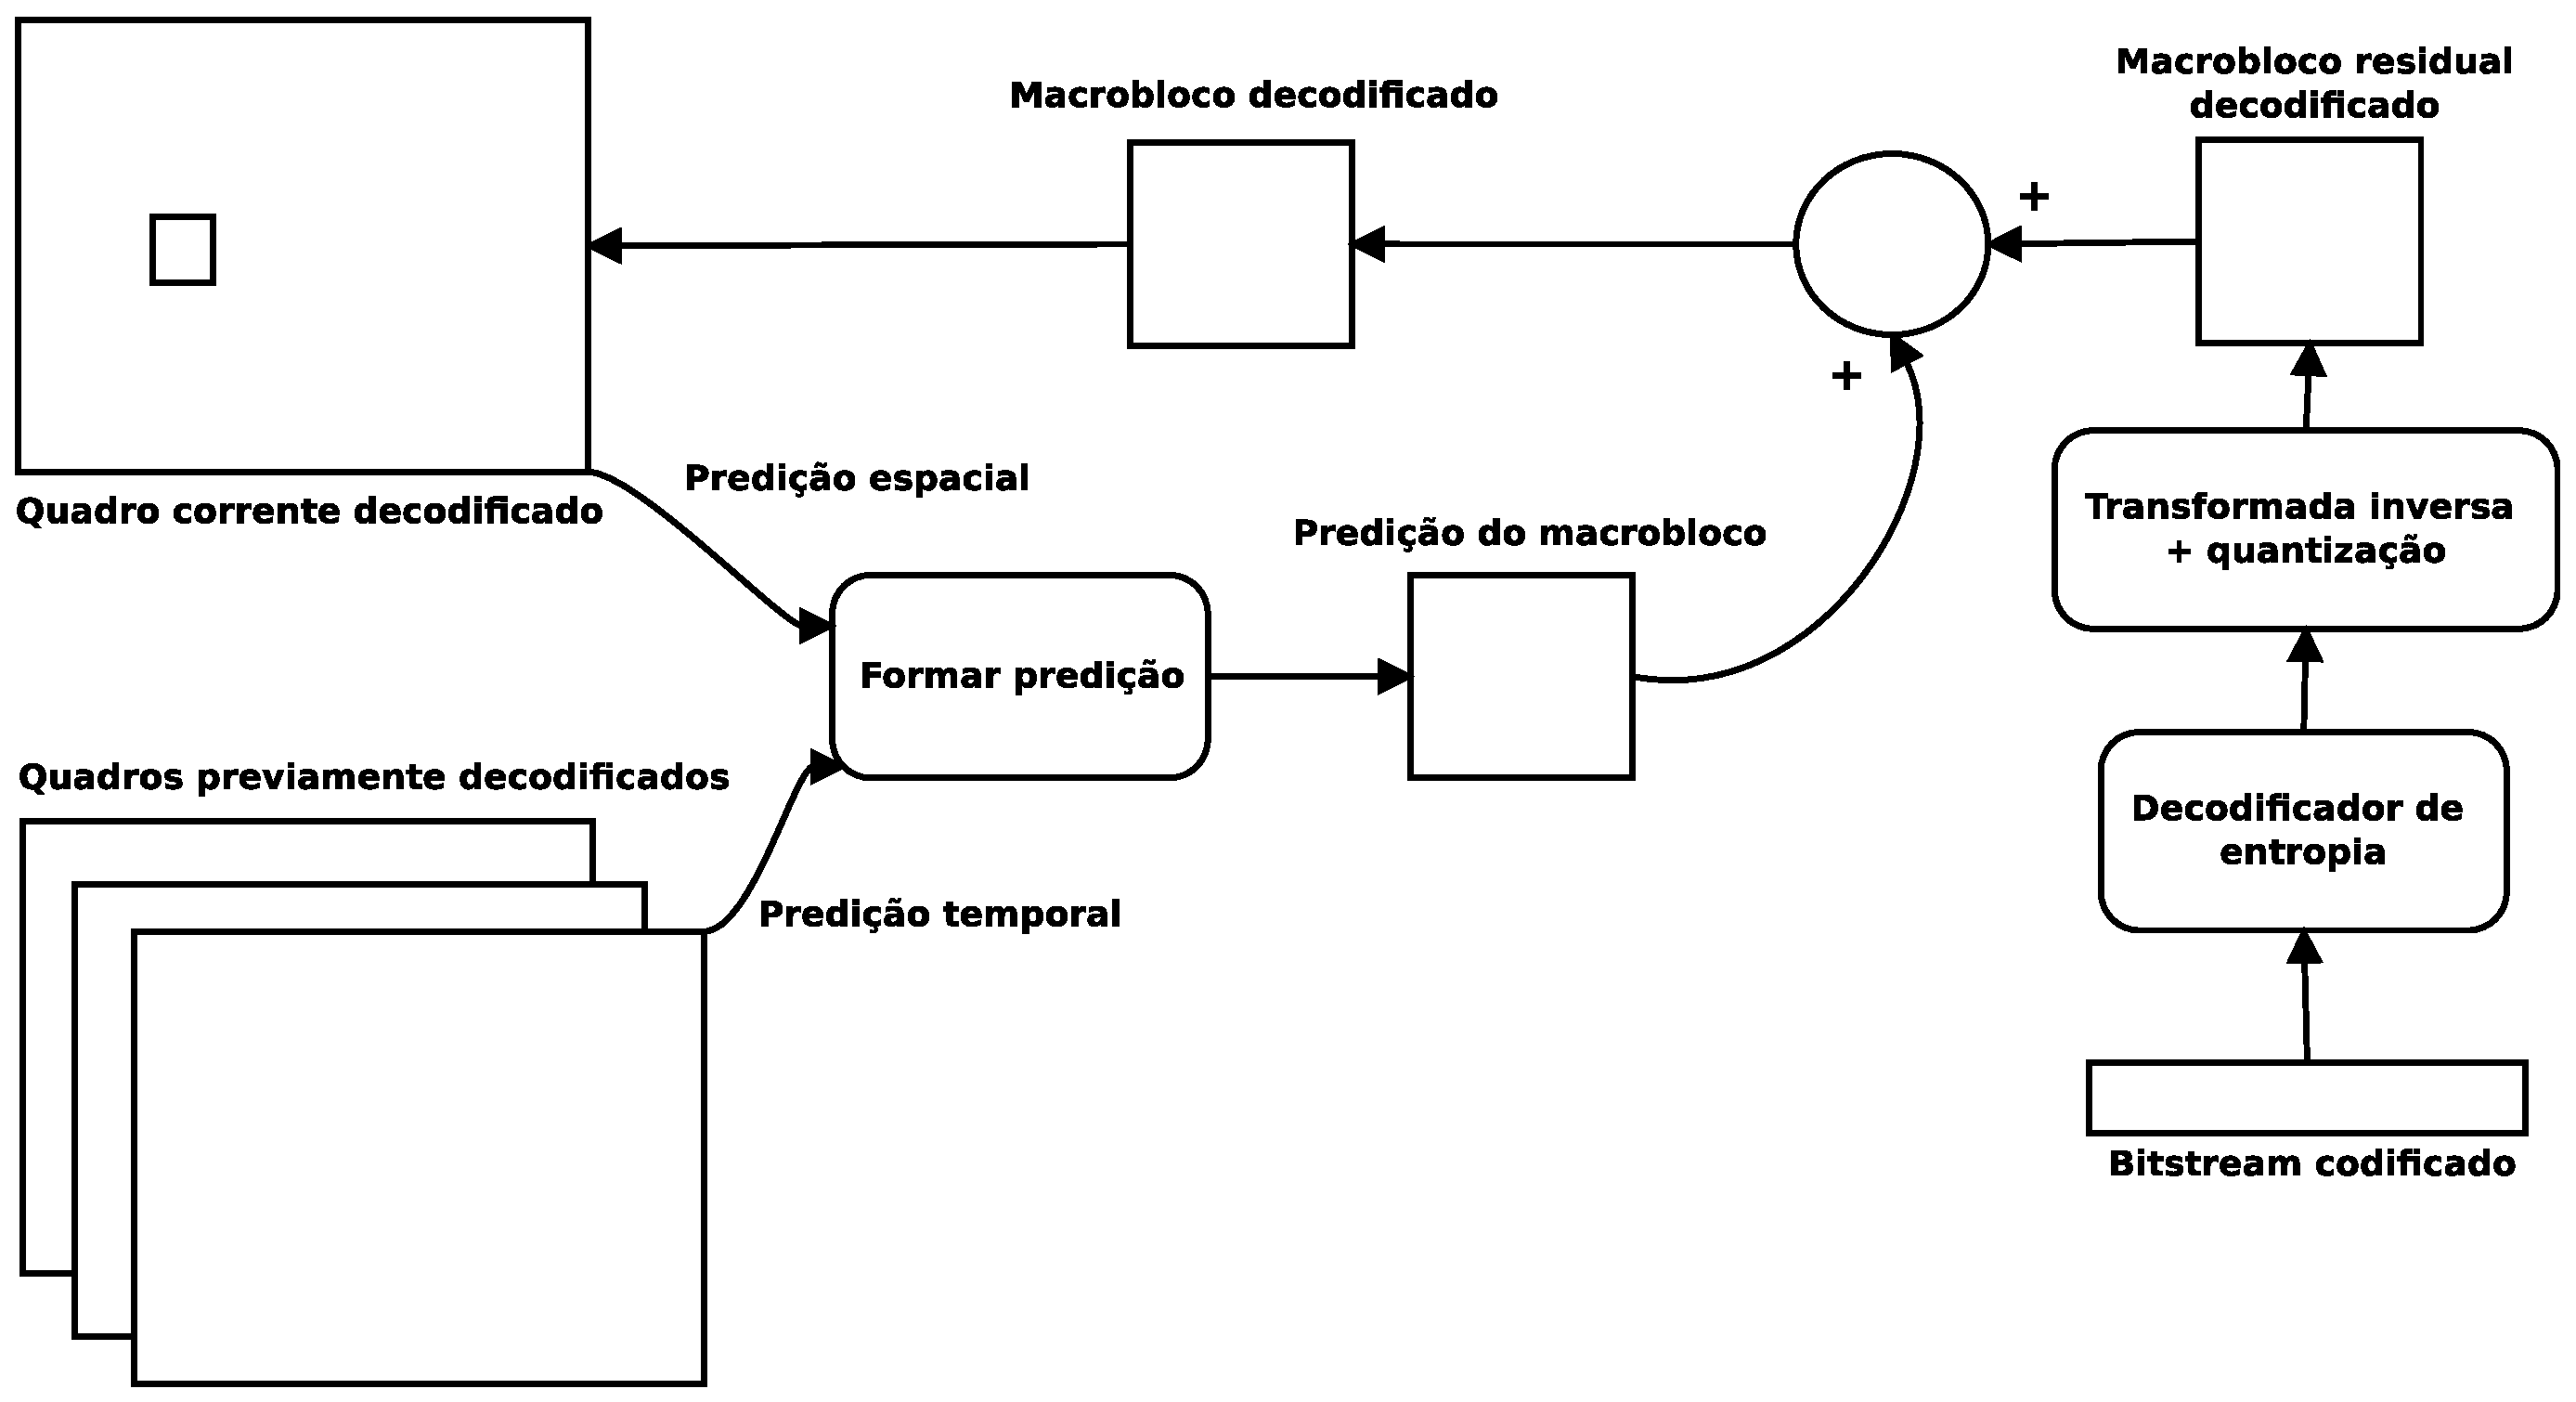
\includegraphics[scale=0.3]{imagens/fig2.eps}
\caption{Típico decodificador H.264}
\label{fig:h264_decoder}
\end{figure}


Todas as informações produzidas pelo codificador tem de ser codificadas e comprimidas em um bitstream que possa ser armazenado/transmitido para ser decodificado posteriormente. Essas informações incluem:

\begin{itemize}
        \item Coeficientes gerados pela transformação (quantizados).
        \item Informação que habilita o decoder a recriar a predição.
        \item Informação da estrutura dos dados comprimidos, e das ferramentas de compressão utilizadas no processo de codificação.
        \item Informação a respeito da sequência de vídeo como um todo.
\end{itemize}

Esses valores e parâmetros, também conhecidos como elementos de sintaxe, são convertidos em código binário utilizando codificação de tamanho variado (VLC) e/ou codificação aritmética. Cada um desses métodos produz uma representação binária eficiente e compacta das informações.


\subsection{Sintaxe Geral}


H.264 provê uma sintaxe clara de como representar o vídeo comprimido e informações relacionadas ao vídeo, essa sintaxe é hierárquica. No nível mais alto, uma sequência H.264 consiste de uma série de "pacotes" ou Network Abstraction Layer Units (NALUs). 

Um NALU (Network Abstraction Layer Unit) contem um RBSP (Raw Byte Sequence Payload), que é uma sequência de bytes contendo os elementos da sintaxe. No H.264 os elementos da sintaxe são códigos binários de tamanho variado, portanto uma sequência de elementos de sintaxe dentro de um NALU não vai necessariamente encaixar em um número integral de bytes, bits com valor zero são adicionados ao final do RBSP para garantir isso.

Cada NALU consiste de um cabeçalho de 1 byte, seguido de um stream de bytes contendo informações de controle ou vídeo codificado. O cabeçalho indica o tipo do NALU e a "importância" dele. NALUs utilizados como referência, por exemplo na predição de quadros futuros, são considerados como de alta prioridade, já que a perda de um desses poderia dificultar o processo de decodificação. Já os NALUs que não são utilizados como referência são considerados como tendo uma prioridade mais baixa. Esse tipo de informação pode ser utilizada para priorizar os NALUs mais importantes no momento da transmissão.


\begin{figure}[H]
\centering
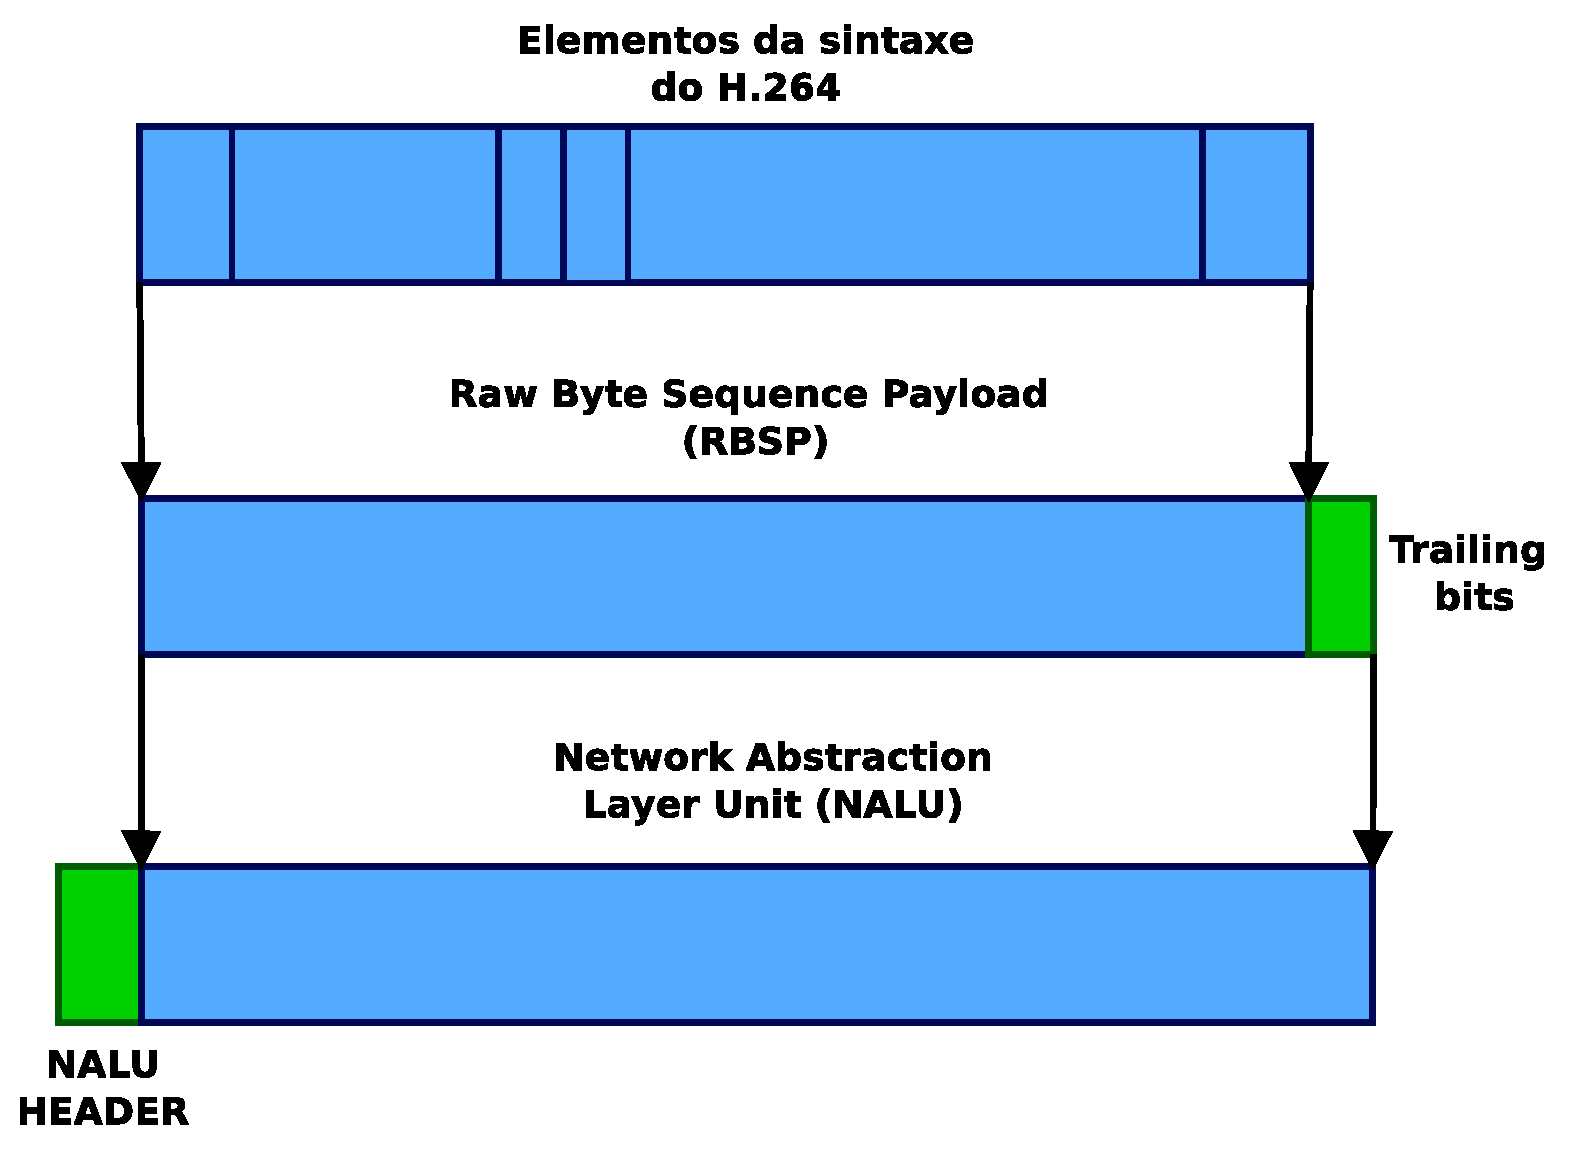
\includegraphics[scale=0.4]{imagens/fig3.eps}
\caption{Encapsulamento de elementos de sintaxe do H.264 em um NALU}
\label{fig:h264_syntax}
\end{figure}


De acordo com \cite{ieeeVideoVol13N7} página 563, um NALU pode ser transmitido usando um protocolo de transporte, onde cada NALU se torna o payload do pacote (orientado a pacote), ou em um stream de bytes, onde cada NALU será transmitido sequencialmente em uma série de bytes (orientado a byte stream), utilizando como prefixo um código de inicio (start code) de 3 bytes indicando que está começando um novo NALU no bitstream. 

Sempre que ocorre de uma sequência de 3 bytes ser similar ao start code, é inserido um emulation prevention byte para prevenir que o decoder confunda essa sequência de bytes com um start code. Quando se utiliza orientação a pacote é desnecessária a utilização do start code e do emulation prevention byte. A sintaxe completa de um NALU pode ser encontrada em \cite{ituh264avc} seção 7.3.1 e sua semântica na seção 7.4.1.


\begin{figure}[H]
\centering
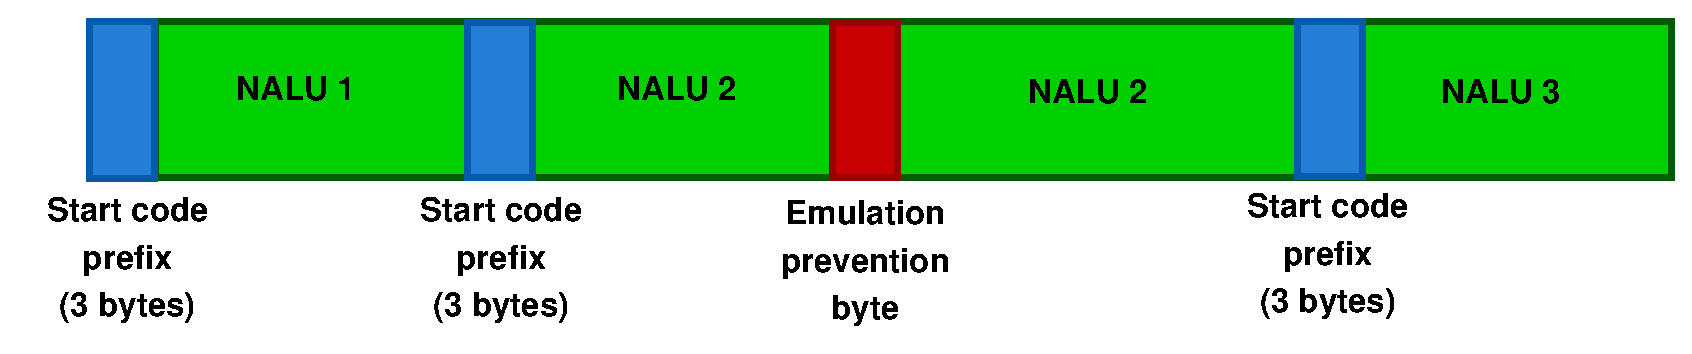
\includegraphics[scale=0.4]{imagens/fig5.eps}
\caption{Exemplo de 3 NALUs sendo transmitidos/armazenados com orientação a bitstream}
\label{fig:h264_nalu_bitstream}
\end{figure}


\begin{figure}[H]
\centering
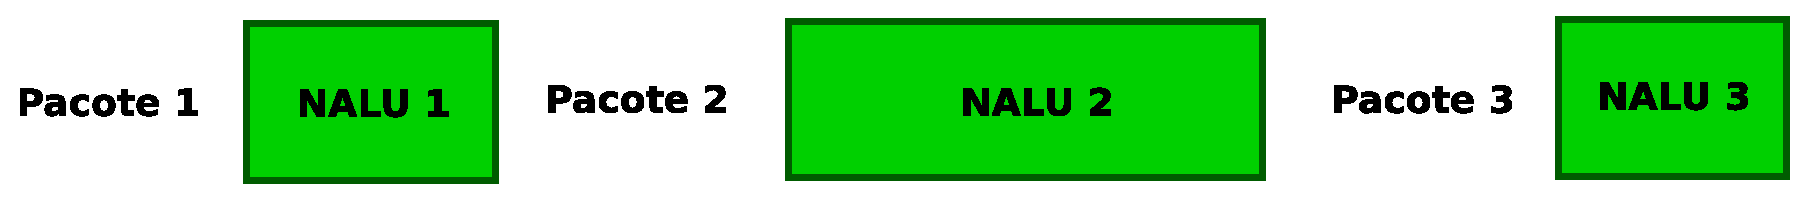
\includegraphics[scale=0.4]{imagens/fig6.eps}
\caption{Exemplo de 3 NALUs sendo transmitidos/armazenados com orientação a pacotes}
\label{fig:h264_nalu_packet}
\end{figure}


Como consta em \cite{ieeeVideoVol13N7} página 564, NALUs podem ser classificados como VCL (pertencem ao video coding layer) ou não-VCL NALUs (não pertencem a Video Coding Layer). 

NALUs VCL possuem as amostras de vídeo (slices) enquanto que NALUs não-VCL possuem informações adicionais associadas ao vídeo como parâmetros (Parameter Sets) que fornecem informações de controle ao decodificador ou SEI (Supplemental Enhancement Information). 

Os Parameter Sets existentes são os SPS (Sequence Parameter Sets), que podem ser aplicados a uma inteira sequência de vídeo, e os PPS (Picture Parameter Sets) que são aplicáveis somente a um ou mais quadros de uma determinada sequência, mas não todos. 


\begin{figure}[H]
\centering
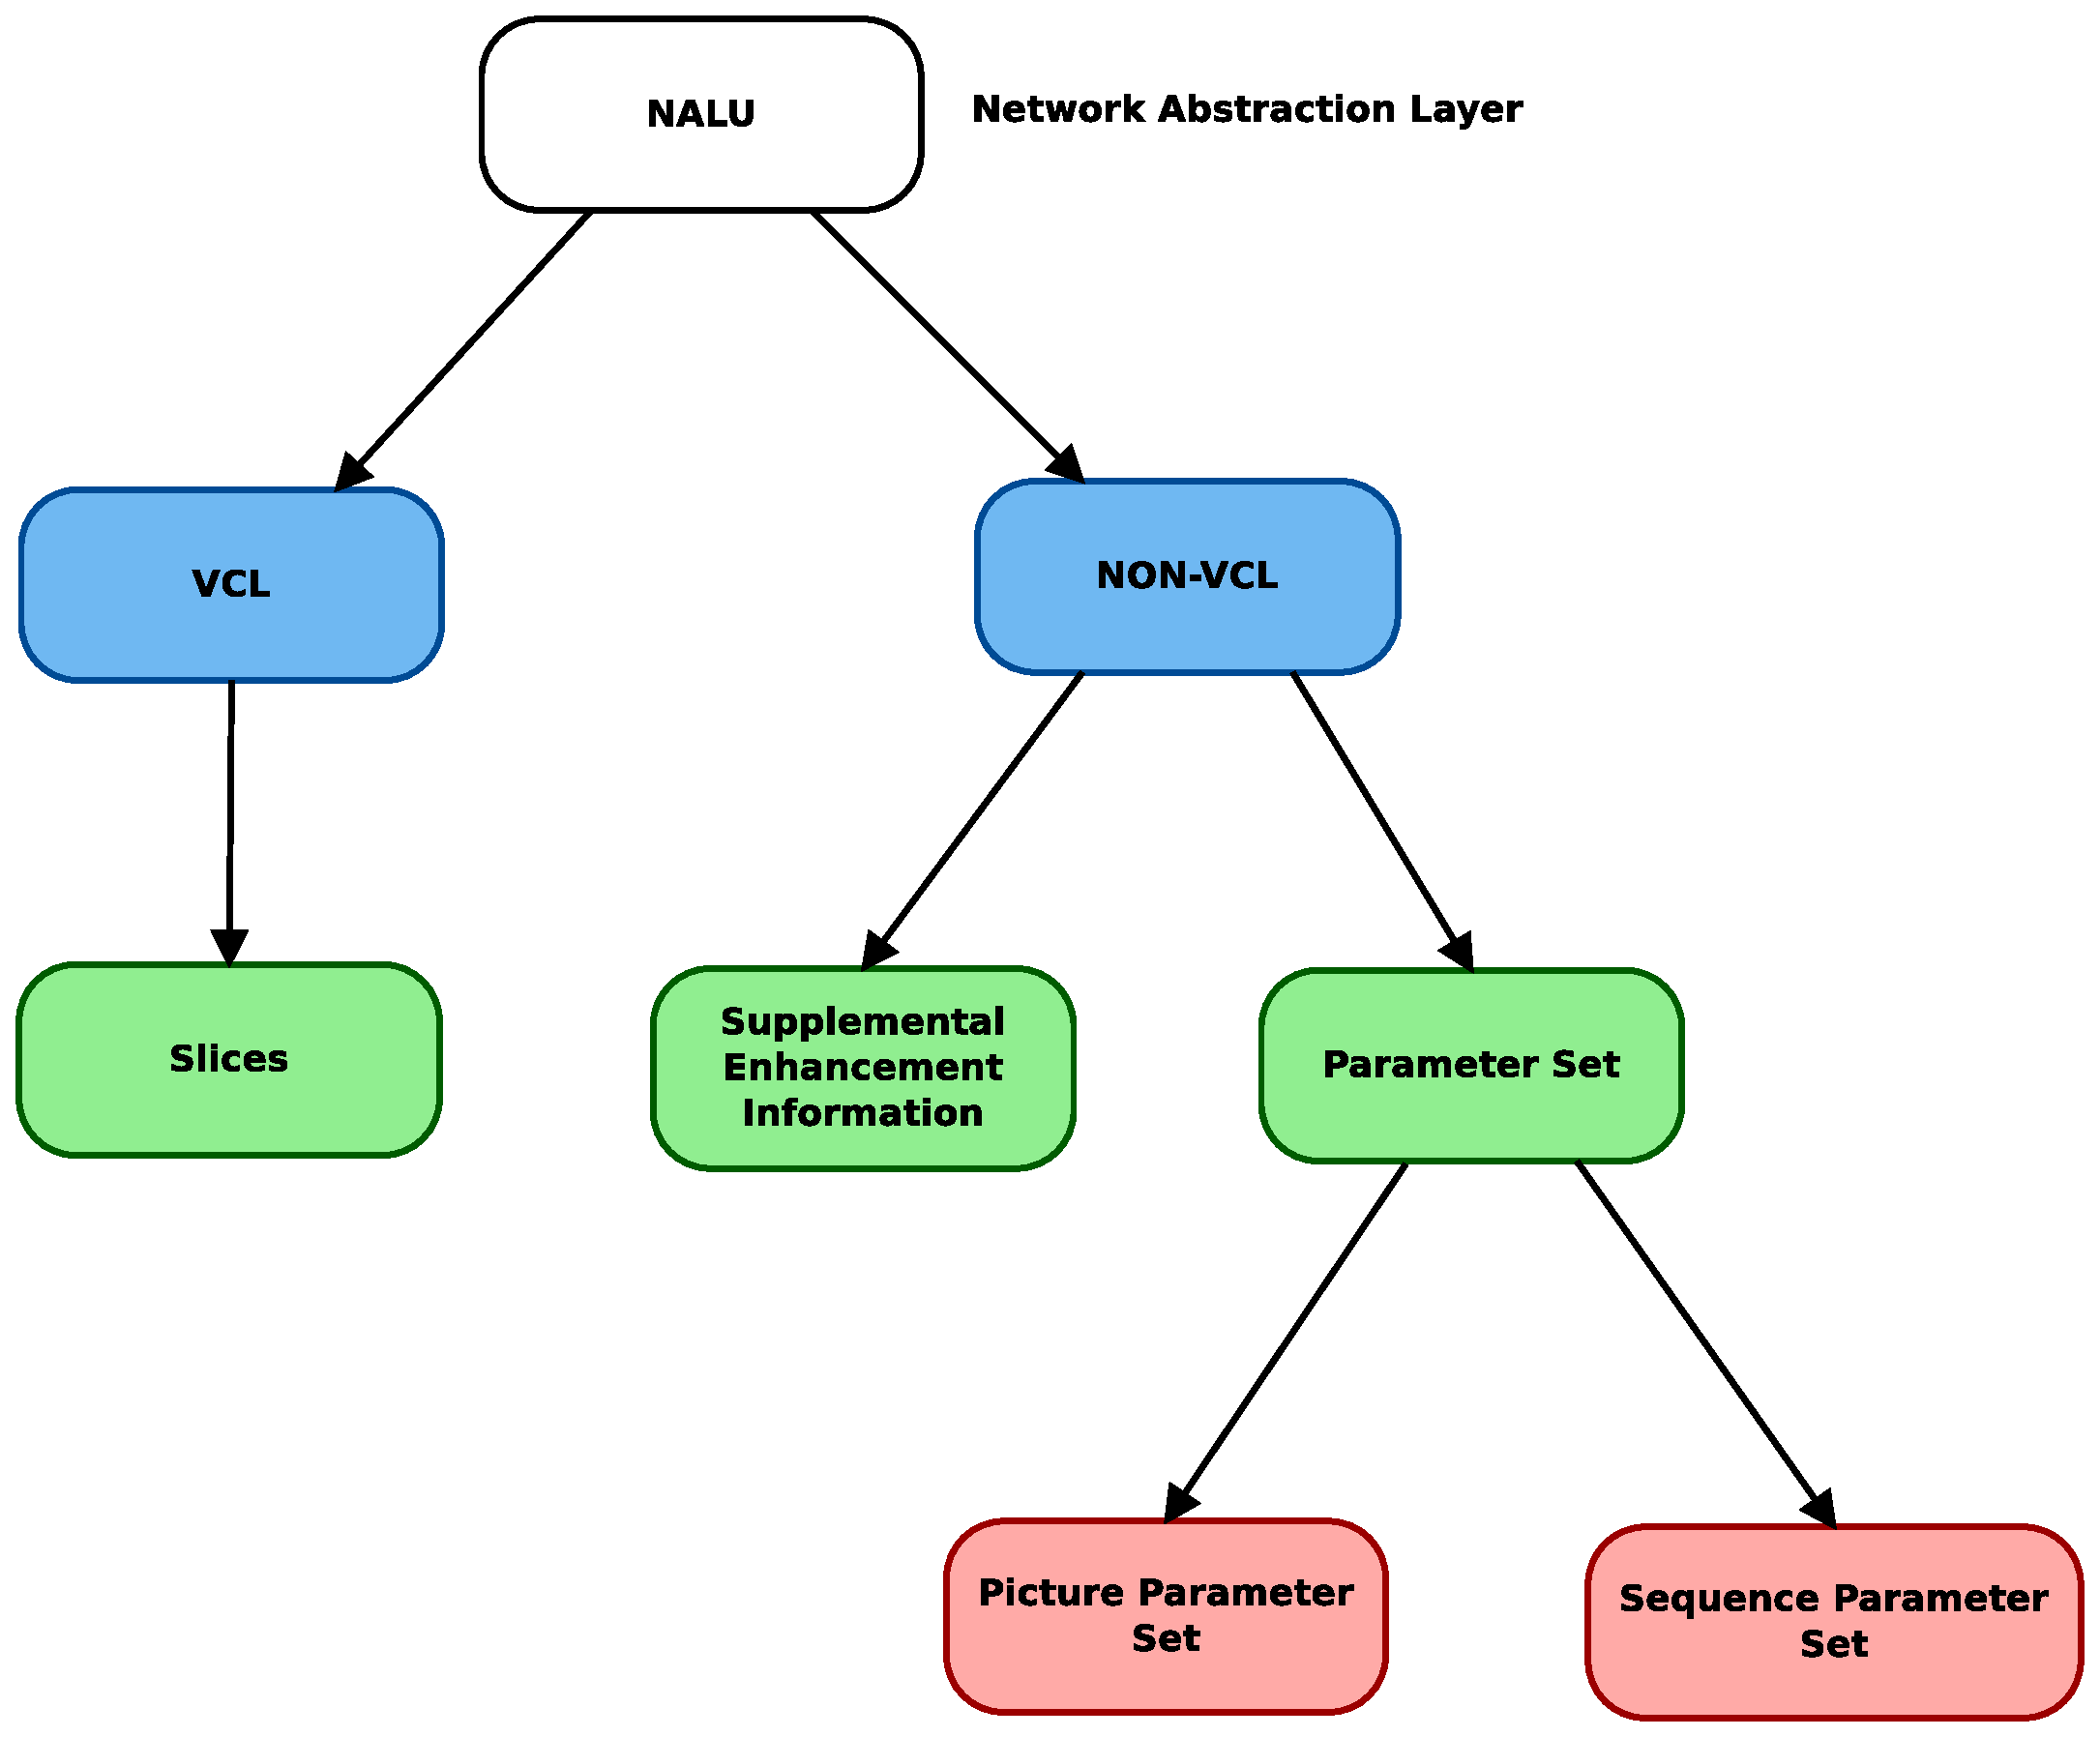
\includegraphics[scale=0.4]{imagens/fig7.eps}
\caption{Possíveis classificações de um NALU}
\label{fig:vcl_nonvcl}
\end{figure}


\subsection{Supplemental Enhancement Information}

Como consta em \cite{ituh264avc} cláusula 7.4.2.3, SEI (Supplemental Enhancement Information) NALUs contêm informações que não são essenciais ao processo de decodificação mas que podem ser utilizadas para auxiliar a decodificação. Um NALU do tipo SEI pode conter uma ou mais mensagens SEI dentro do seu RBSP. A sub-cláusula 7.3.2.3 define a sintaxe do RBSP de um NALU do tipo SEI, mais informações sobre SEI podem ser encontrados no anexo D da recomendação.


\begin{figure}[H]
\centering
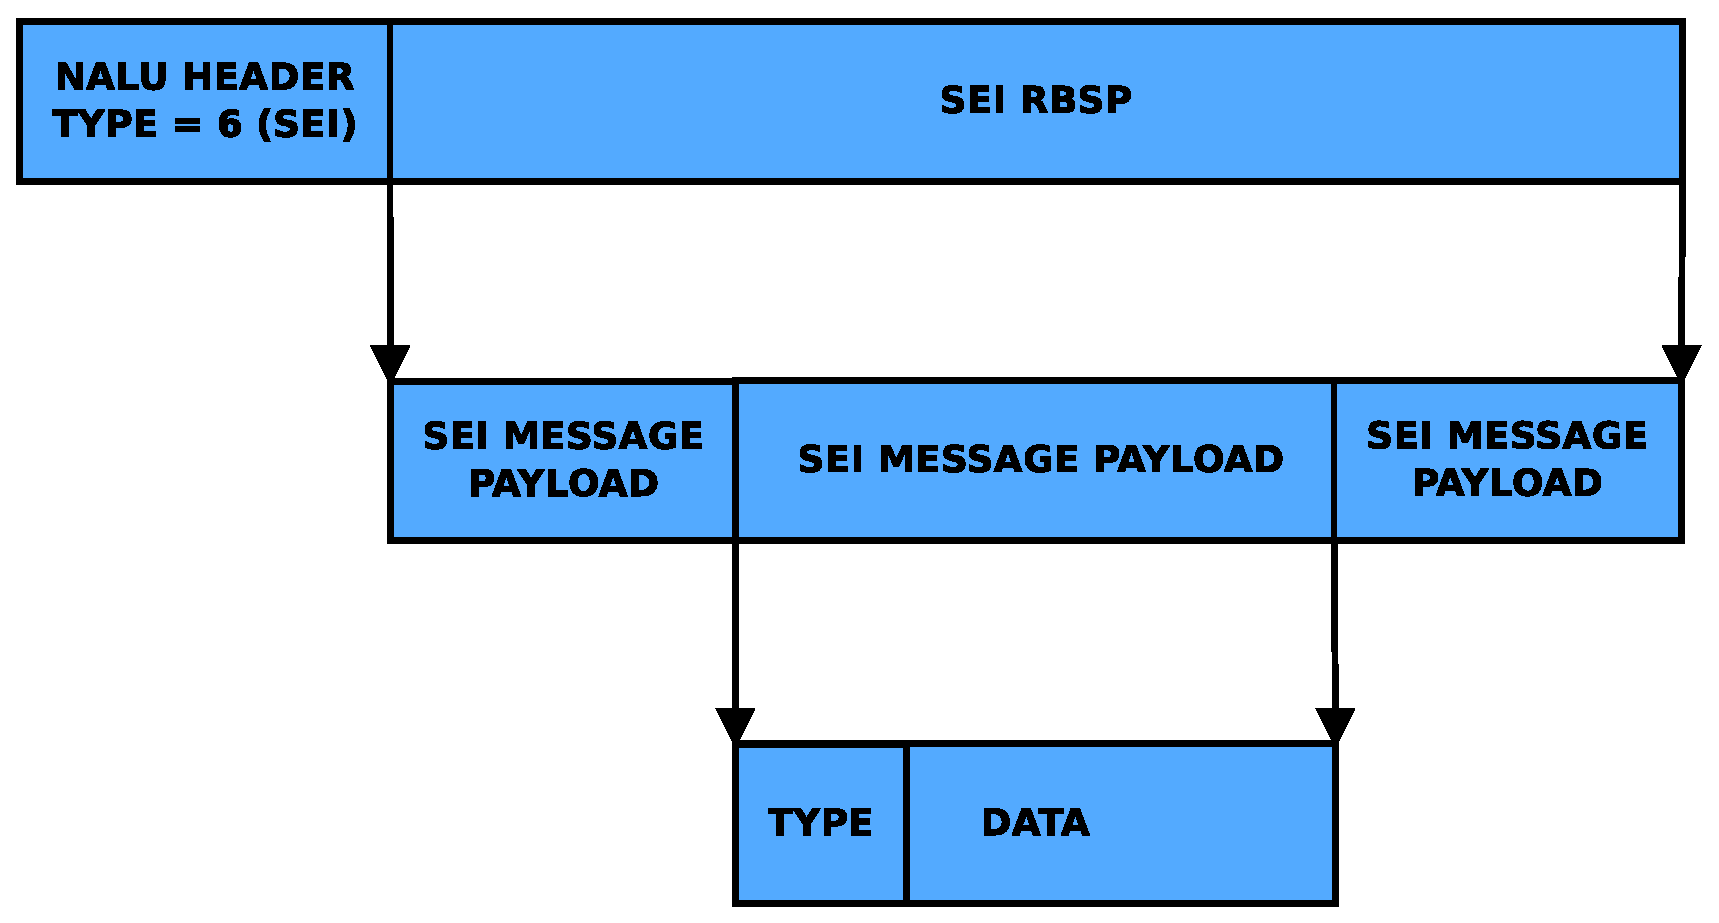
\includegraphics[scale=0.5]{imagens/fig4.eps}
\caption{Exemplo de mensagens SEI encapsuladas em um SEI NALU}
\label{fig:sei_nalu}
\end{figure}


Não existe um limite máximo no tamanho de um SEI NALU, porém existem algumas limitações de buffer que podem resultar em um limite implícito no tamanho do SEI NALU (tabela A.1 do anexo A da \cite{ituh264avc} traz os limites que podem existir de acordo com o nível/perfil que o codificador implemente).

A sub-cláusula 7.3.2.3.1 da recomendação \cite{ituh264avc} define a sintaxe de uma mensagem SEI e a sub-cláusula 7.4.2.3.1 define a sua semântica, nestas sub-cláusulas pode se encontrar informações mais detalhadas de como o decodificador consegue obter o tamanho das mensagens SEI.

Uma mensagem SEI é composta basicamente do tipo do payload e o próprio payload. Normalmente as mensagens SEI são utilizadas para auxiliar o processo de decodificação, por isso existem vários tipos de mensagens pré-definidas. 

Existem dois tipos de mensagem SEI \textit{UserData}, a registrada e a não registrada, ambas podem possuir dados que não são definidos na recomendação \cite{ituh264avc}. Na mensagem SEI \textit{UserData} registrada a mensagem deve ser precedida por um código registrado na ITU-T e a mensagem deve seguir a sintaxe e a semântica estipuladas por esse código informado. 

Já a mensagem SEI \textit{UserData} não registrada necessita de um UUID precedendo a mensagem e o conteúdo da mensagem não precisa obedecer nenhuma sintaxe ou semântica específica. A sintaxe do payload de uma mensagem SEI \textit{UserData} não registrada pode ser encontrada em \cite{ituh264avc} na seção D.1.6 e a definição semântica na seção D.2.6.

Uma lista completa de todos os tipos de mensagens SEI se encontra em \cite{ituh264avc} na seção D.1.


\subsection{Software de referência H.264/AVC}

O software de referência utilizado no presente projeto é desenvolvido pelo JVT (Joint Video Team) e hospedado pelo Instituto Fraunhofer para telecomunicações, Instituto Heinrich Hertz. Esta implementação será utilizada por ela ser referência para pesquisas e verificação de conformidade com a norma. 

A versão utilizada é a 17.2, o download da mesma pode ser realizado gratuitamente em http://iphome.hhi.de/suehring/tml/download, todos os módulos são bem divididos e possuem boa documentação. O software consiste basicamente de um codificador (\textit{lencod}) que codifica um arquivo de vídeo raw para o formato H.264 e de um decodificador (\textit{ldecod}) que decodifica um arquivo H.264 em um arquivo de vídeo raw. Algumas funções de uso comum se encontram no módulo \textit{lcommon}.


\section{Classificador Haar - OpenCV}


\subsection{Introdução}

OpenCV inclui diversas implementações de algoritmos de aprendizagem de máquina (uma lista completa dos algoritmos disponíveis encontra-se em \cite{learningOpenCV} páginas 462 e 463), que é um sub-campo da inteligência artificial que visa transformar dados brutos em informação, tornando possível que a máquina responda a perguntas como: Que outra informação é similar a esta? Existe um carro nessa imagem?

Um desses algoritmos de aprendizagem de máquina é o classificador Haar, esse algoritmo é uma implementação da técnica conhecida como detector Viola-Jones \cite{rapidObjectDetectionViola01} e que depois foi estendido por Rainer Lienhart e Jochen Maydt \cite{extendedSetHaarFeatures02} para utilizar recursos diagonais. Ele é um classificador supervisionado (para mais informações sobre tipos de classificadores veja \cite{learningOpenCV} páginas 460 e 461), ou seja, após treiná-lo é necessário apenas fornecer a imagem ao classificador e ele irá rotular ela como contendo ou não contendo o objeto de interesse.


\subsection{Teoria do classificador Viola-Jones}

O detector Viola-Jones utiliza uma forma de AdaBoost (\cite{learningOpenCV} página 497) mas o organiza como uma cascata de nodos, onde cada nodo desse é um classificador "Multitree AdaBoosted", desenvolvido para ter uma alta (digamos 99,9\%) taxa de detecção (poucos falsos negativos), ás custas de uma baixa (perto de 50\%) taxa de rejeição (grande quantidade de falsos positivos).

A cascata de nodos funciona como uma cascata de rejeição, para cada nodo na cascata, um "não pertence a classe" encerra a computação e o algoritmo responderá que não existe o objeto de pesquisa na região determinada para busca.  A região só é classificada como possuindo um objeto de determinada classe se a computação ocorrer com sucesso por toda a cascata. 

Em casos onde o objeto de interesse é raro (por exemplo uma face em uma foto), cascatas de rejeição aceleram o processo de busca por um objeto, já que a maior parte das regiões de busca será marcada como não possuindo o objeto rapidamente, sem ter de percorrer a maior parte da cascata. Em cada nodo da cascata de rejeição existe um conjunto de classificadores fracos, que são árvores de decisão. O conjunto de árvores em cada nodo é acelerado com a técnica de Boosting (mais informações sobre a técnica de Boosting podem ser encontradas em \cite{learningOpenCV} página 495).

 Essas árvores normalmente possuem profundidade um, sendo também chamadas de \textit{decision stumps}, são o caso mais simples de árvores de decisão o qual consiste de um único nodo de decisão e duas folhas. Cada "decision stump" deve tomar apenas uma decisão, da seguinte forma: "Está o valor V de um determinado recurso R acima ou abaixo de um limite L"; Nesse caso um "sim" indica que o objeto de interesse está presente, um "não" indica a sua ausência.

\begin{displaymath}
   f{i} = \left\{
     \begin{array}{lr}
       +1 & : V{i} \geq T{i} \\
       -1 & : V{i} < T{i} 
     \end{array}
   \right.
\end{displaymath}

A quantidade de recursos Haar que o classificador Viola-Jones utiliza em cada classificador fraco pode ser configurado no momento do treinamento, normalmente se utiliza apenas um recurso (uma árvore com apenas uma divisão) ou no máximo 3 recursos. Incrementar esses classificadores iterativamente (técnica de Boosting) constrói um classificador que é a soma ponderada dos classificadores fracos. O classificador Viola-Jones usa a seguinte função de classificação:

\begin{equation}
F = sinal(w{1}f{1} + w{2}f{2} + ... + w{n}f{n})
\end{equation}

A função sinal retorna -1 se o resultado da soma for menor ou igual a 0,0, do contrário retorna +1. Ao analisar pela primeira vez o conjunto de dados, nós aprendemos o limite l1 de f1 que melhor classifica a entrada. A técnica de Boosting utiliza os erros para realizar o calculo ponderado de w1. Cada vetor de recursos é reavaliado como tendo menos peso (se ele foi classificado corretamente) ou mais peso (se ele foi classificado incorretamente). 

Pode parecer estranho diminuir o peso do vetor de dados quando ele é classificado corretamente, e aumentar o peso quando a classificação falha. A razão do treinamento ocorrer assim é que a técnica de Boosting tem como objetivo corrigir os pontos onde existem "problemas" e ignorar os pontos que já funcionam bem. Depois que o nodo é ensinado, os dados sobreviventes da parte superior da cascata são usados para treinar o próximo nodo, e assim por diante.

Um detalhe importante é o uso de recursos Haar como entrada do algoritmo, em vez de dados brutos. Esses recursos Haar são basicamente um limite aplicado às somas e diferenças de regiões retangulares da imagem. Para acelerar o cálculo desses recursos é utilizada a técnica de imagem integral (para mais detalhes veja \cite{learningOpenCV} página 182) que acelera o cálculo do valor de regiões retangulares e dessas mesmas regiões rotacionadas em 45 graus. 

Viola e Jones organizaram cada grupo classificador boosted em nodos, formando uma cascata de rejeição, como mostrado na figura ~\ref{fig:cascata_rejeicao_haar}. Na figura , cada nodo F contem uma inteira cascata boosted de grupos de \textit{decision stumps} (ou árvores) treinadas utilizando recursos Haar. Normalmente os nodos são ordenados do menos complexo ao mais complexo, assim o custo computacional é minimizado (os nodos mais simples são executados primeiro) ao analisar regiões da imagem que com certeza não possuem o objeto de interesse.

\begin{figure}[H]
\centering
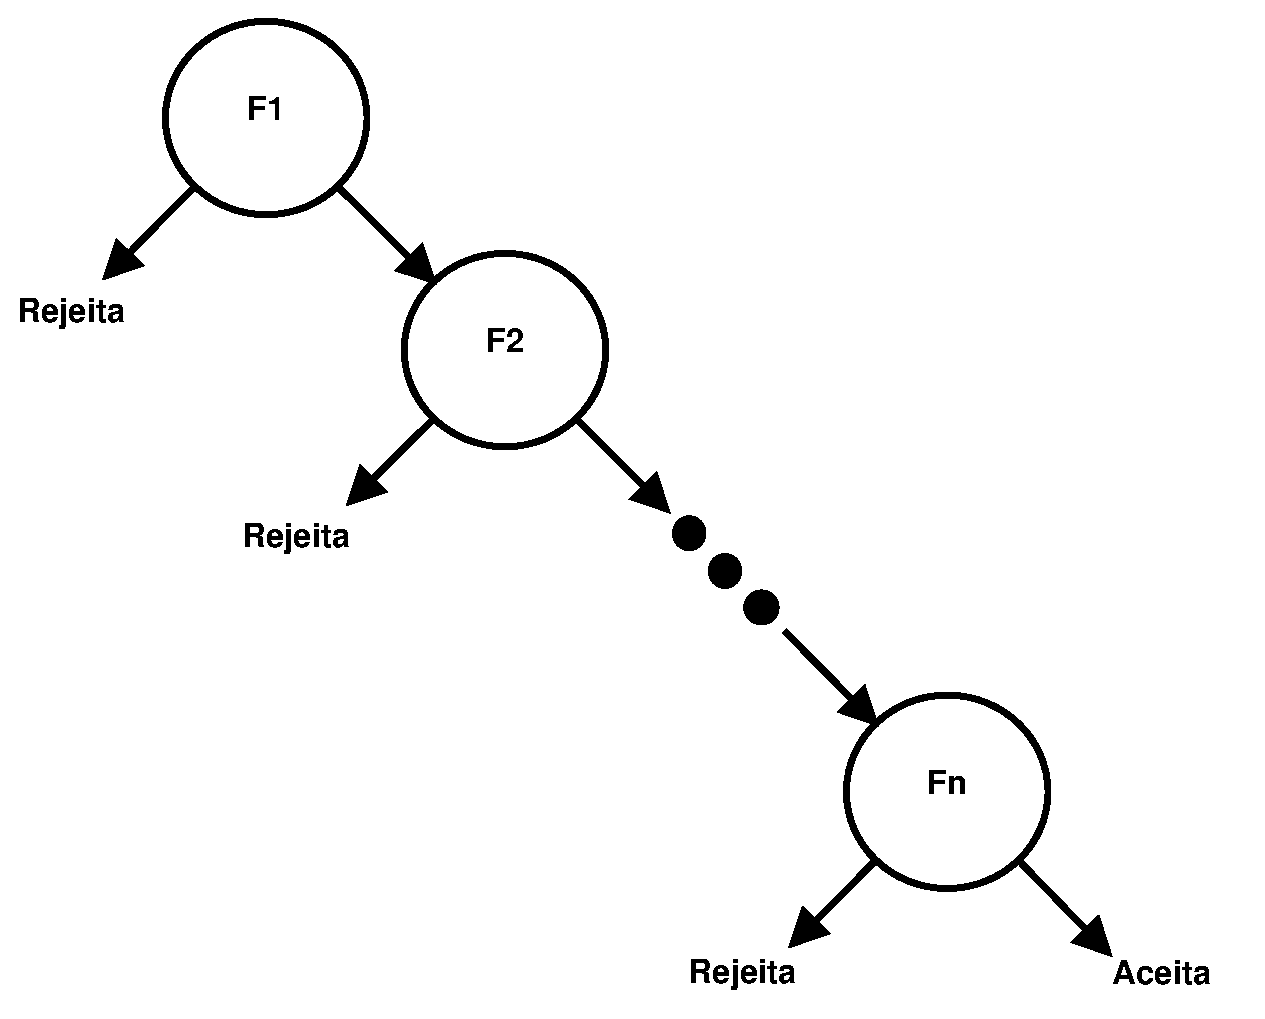
\includegraphics[scale=0.6]{imagens/fig8.eps}
\caption{Cascata de rejeição utilizada no classificador Viola-Jones: Cada nodo representa um classificador "Multitree AdaBoosted" treinado para raramente perder o objeto de interesse, rejeitando porém apenas uma pequena parte das regiões que não representam o objeto de interesse. Até chegar o final da cascata a maior parte das regiões que não representam o objeto de interesse já foram descartadas. }
\label{fig:cascata_rejeicao_haar}
\end{figure}


\subsection{Uso do classificador}

O classificador Haar funciona bem em objetos como faces frontais, olhos, boca, traseira de carros, lateral de carros, frente de carros; Mas objetos como o perfil de um rosto (ou qualquer outro objeto em que o contorno seja a característica principal de identificação), já não funciona tão bem, principalmente porque essa perspectiva insere variações no padrão que os recursos em forma de bloco do Haar não conseguem lidar muito bem. 

Por exemplo, para modelar a curva de um rosto visto de lado (seu contorno) é necessário inserir no modelo informações a respeito do fundo da imagem, para realizar essa modelagem de maneira adequada seria necessário um conjunto de treinamento muito maior, com diferentes fundos na imagem, ou rostos de lado com fundos diferentes do modelado seriam rejeitados. Ou seja, o contorno de um objeto é difícil de modelar nesse classificador porque os recursos Haar funcionam em bloco, dessa maneira o classificador é obrigado a aprender as variações do fundo da imagem que formam a borda do objeto.

Para treinar o classificador é necessário ter um grande conjunto de dados, com boa qualidade, bem segmentado, para detecção de objetos rígidos onde o contorno não é a principal característica do objeto. O treinamento desse classificador é lento, porém graças a modelagem em cascata de rejeição ele é bem rápido para realizar a detecção do objeto em si.

Por grande conjunto de dados entende-se milhares de imagens com o objeto de interesse e dezenas de milhares de objetos sem o objeto de interesse. Por boa qualidade dos dados entende-se que os dados não devem conter o mesmo objeto em perspectivas diferentes, para cada perspectiva diferente é melhor treinar um classificador especifíco para aquela perspectiva. 

Por bem segmentado entende-se imagens que representam corretamente o objeto sem variações desnecessárias, isso faria com que o classificador corrigisse essa variação fictícia, levando a resultados imprecisos. Por exemplo, ao treinar o classificador para detectar faces frontais, se a localização dos olhos no rosto variar demais (algo fora do normal) o classificador vai assumir que a localização dos olhos não é fixa e que é normal que os olhos possam estar em qualquer posição, isso degrada muito o desempenho já que o classificador precisa se ajustar a fatores que não existem nos dados reais.

